%%%%%%%%%%%%%%%%%%%%%%%%%%%%%%%%%%%%
% Slide options
%%%%%%%%%%%%%%%%%%%%%%%%%%%%%%%%%%%%

% Option 1: Slides with solutions

\documentclass[t,compress,mathserif]{beamer}
\newcommand{\soln}[1]{\textit{#1}}
\newcommand{\solnGr}[1]{#1}

% Option 2: Handouts without solutions

%\documentclass[11pt,containsverbatim,handout]{beamer}
%\usepackage{pgfpages}
%\pgfpagesuselayout{4 on 1}[letterpaper,landscape,border shrink=5mm]
%\newcommand{\soln}[1]{ }
%\newcommand{\solnGr}{ }


%%%%%%%%%%%%%%%%%%%%%%%%%%%%%%%%%%%%
% Style
%%%%%%%%%%%%%%%%%%%%%%%%%%%%%%%%%%%%

\def\chp5@path{../../Chp 5}
\input{../../lec_style.tex}

%%%%%%%%%%%%%%%%%%%%%%%%%%%%%%%%%%%%
% Preamble
%%%%%%%%%%%%%%%%%%%%%%%%%%%%%%%%%%%%

\title[Lecture 18]{MA213: Lecture 18}
\subtitle{Module 3: Foundations for inference}
\author{OpenIntro Statistics, 4th Edition}
\institute{$\:$ \\ {\footnotesize Based on slides developed by Mine \c{C}etinkaya-Rundel of OpenIntro. \\
The slides may be copied, edited, and/or shared via the \webLink{http://creativecommons.org/licenses/by-sa/3.0/us/}{CC BY-SA license.} \\
Some images may be included under fair use guidelines (educational purposes).}}
\date{}


%%%%%%%%%%%%%%%%%%%%%%%%%%%%%%%%%%%%
% Begin document
%%%%%%%%%%%%%%%%%%%%%%%%%%%%%%%%%%%%

\begin{document}


%%%%%%%%%%%%%%%%%%%%%%%%%%%%%%%%%%%%
% Title page
%%%%%%%%%%%%%%%%%%%%%%%%%%%%%%%%%%%%

{
\addtocounter{framenumber}{-1} 
{\removepagenumbers 
\usebackgroundtemplate{\includegraphics[width=\paperwidth]{../../OpenIntro_Grid_4_3-01.jpg}}
\begin{frame}

\hfill \includegraphics[width=20mm]{../../oiLogo_highres}

\titlepage

\end{frame}
}
}


%%%%%%%%%%%%%%%%%%%%%%%%%%%%%%%%%%%%
% Recap/Agenda 
%%%%%%%%%%%%%%%%%%%%%%%%%%%%%%%%%%%%
% TODO better formatting
\begin{frame}
    \frametitle{Module 3: Foundations for inference}
    \begin{itemize}
        \item \hl{Previously: }Confidence intervals for a proportion (Chapter 5.2)
        \item \hl{This time: }Hypothesis testing for a proportion (Chapter 5.3)
        \item \hl{Reading: }Chapter 6.1 for next time
        \item \hl{Deadlines/Announcements: }
        \begin{itemize}
        \item HW 6 due today
        \item Quiz 2 tomorrow in class (not discussion)
        \item Prof Stephen Office hours: Today 12:15-1:30pm, *no OH on Thursday*
        \end{itemize}
    \end{itemize}
    
\end{frame}

            
%%%%%%%%%%%%%%%%%%%%%%%%%%%%%%%%%%%%
% Learning objectives:
%%%%%%%%%%%%%%%%%%%%%%%%%%%%%%%%%%%%
\begin{frame}
    \frametitle{Learning Objectives}
    \begin{itemize}
        \item \textbf{M3 LO3: Calculate and Interpret Standard Error:} Calculate the standard error for proportions and interpret it as a measure of sampling variability.
        \item \textbf{M3, LO4: Explain Hypothesis Testing and Its Limitations:} Discuss the use cases and potential issues with hypothesis testing, including the interpretation of results.
        \item \textbf{M3, LO5: Understand Errors and Significance Levels:} Identify Type I and Type II errors and explain how they are influenced by changes in the significance level.
    \end{itemize}
\end{frame}


%%%%%%%%%%%%%%%%%%%%%%%%%%%%%%%%%%%%
% Sections
%%%%%%%%%%%%%%%%%%%%%%%%%%%%%%%%%%%%

%%%%%%%%%%%%%%%%%%%%%%%%%%%%%%%%%%%%

\section{Hypothesis testing for a proportion}

%%%%%%%%%%%%%%%%%%%%%%%%%%%%%%%%%%%%

\subsection{Hypothesis testing framework}

%%%%%%%%%%%%%%%%%%%%%%%%%%%%%%%%%%%%

\begin{frame}
\frametitle{Remember when...}

Gender discrimination experiment:

{\footnotesize
\begin{tabular}{ll  cc c} 
  		&				& \multicolumn{2}{c}{\textit{Promotion}} \\
\cline{3-4}
							&			& Promoted	& Not Promoted 	& Total	\\
\cline{2-5}
\multirow{2}{*}{\textit{Gender	}}	&Male 		& 21	 	& 3		& 24 	\\
							&Female		& 14	 	& 10 	 	& 24 \\
\cline{2-5}
							&Total		& 35		& 13		& 48 \\
\end{tabular}
}

\pause

\[ \hat{p}_{males} = 21 / 24 \approx 0.88 ~ \text{ and } ~ \hat{p}_{females} = 14 / 24 \approx 0.58 \]

\pause

Possible explanations:
\begin{itemize}
\item Promotion and gender are \hl{independent}, no gender discrimination, observed difference in proportions is simply due to chance. $\rightarrow$ \orange{null} - {\small (nothing is going on)}
\item Promotion and gender are \hl{dependent}, there is gender discrimination, observed difference in proportions is not due to chance. $\rightarrow$ \orange{alternative} - {\small (something is going on)}

\end{itemize}

\end{frame}

%%%%%%%%%%%%%%%%%%%%%%%%%%%%%%%%%%%%

\begin{frame}
\frametitle{Result}

\begin{center}
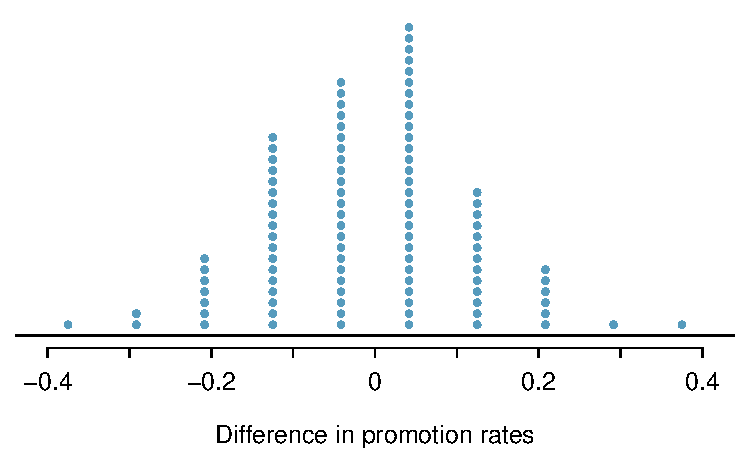
\includegraphics[width=0.75\textwidth]{\chp5@path/5-3_ht_prop/figures/discRandDotPlot/discRandDotPlot}
\end{center}

\pause

Since it was quite unlikely to obtain results like the actual data or something more extreme in the simulations (male promotions being 30\% or more higher than female promotions), we decided to reject the null hypothesis in favor of the alternative.

\end{frame}

%%%%%%%%%%%%%%%%%%%%%%%%%%%%%%%%%%%%

\begin{frame}
\frametitle{Recap: hypothesis testing framework}

\begin{itemize}
\item We start with a \hl{null hypothesis ($H_0$)} that represents the status quo.
\pause
\item We also have an \hl{alternative hypothesis ($H_A$)} that represents our research question, i.e. what we're testing for.
\pause
\item We conduct a hypothesis test under the assumption that the null hypothesis is true, either via simulation or traditional methods based on the central limit theorem (coming up next...).
\pause
\item If the test results suggest that the data do not provide convincing evidence for the alternative hypothesis, we stick with the null hypothesis. If they do, then we reject the null hypothesis in favor of the alternative.
\end{itemize}
\pause
We'll formally introduce the hypothesis testing framework using an example on testing a claim about a proportion.

\end{frame}

%%%%%%%%%%%%%%%%%%%%%%%%%%%%%%%%%%%

 \subsection{Testing hypotheses using confidence intervals} 

%%%%%%%%%%%%%%%%%%%%%%%%%%%%%%%%%%%%

\begin{frame}
\frametitle{Testing hypotheses using confidence intervals}

{\small \dq{Earlier we calculated a 95\% confidence interval for the proporton of American Facebook users who think Facebook categorizes their interests accurately as 64\% to 67\%. Based on this confidence interval, do the data support the hypothesis that majority of American Facebook users think Facebook categorizes their interests accurately.}}

\pause

\begin{itemize}

\item The associated hypotheses are:
\begin{itemize}
\item[$H_0$:] $p = 0.50$: 50\% of American Facebook users think Facebook categorizes their interests accurately
\item[$H_A$:] $p > 0.50$: More than 50\% of American Facebook users think Facebook categorizes their interests accurately
\end{itemize}

\pause

\item Null value is not included in the interval $\rightarrow$ reject the null hypothesis.

\pause

\item This is a quick-and-dirty approach for hypothesis testing, but it doesn't tell us the likelihood of certain outcomes under the null hypothesis (p-value).

\end{itemize}

\end{frame}

%%%%%%%%%%%%%%%%%%%%%%%%%%%%%%%%%%%%

\section{R Demonstration: Experiments}

%%%%%%%%%%%%%%%%%%%%%%%%%%%%%%%%%%%%

\section{Edfinity quiz: Confidence levels}

%%%%%%%%%%%%%%%%%%%%%%%%%%%%%%%%%%%%

\subsection{Decision errors}

%%%%%%%%%%%%%%%%%%%%%%%%%%%%%%%%%%%%

\begin{frame}
\frametitle{Decision errors}

\begin{itemize}

\item Hypothesis tests are not flawless.

\item In the court system innocent people are sometimes wrongly convicted and the guilty sometimes walk free.

\item Similarly, we can make a wrong decision in statistical hypothesis tests as well. 

\item The difference is that we have the tools necessary to quantify how often we make errors in statistics.

\end{itemize}

\end{frame}

%%%%%%%%%%%%%%%%%%%%%%%%%%%%%%%%%%%%

\begin{frame}
\frametitle{Decision errors (cont.)}

There are two competing hypotheses: the null and the alternative. In a hypothesis test, we make a decision about which might be true, but our choice might be incorrect. \\

\pause

\begin{center}
\begin{tabular}{l l | c c}
\multicolumn{2}{c}{} & \multicolumn{2}{c}{\textbf{Decision}} \\
& & fail to reject $H_0$ &  reject $H_0$ \\
  \cline{2-4}
& $H_0$ true & \onslide<3->{\green{$\checkmark$}} &  \onslide<5->{\orange{Type 1 Error}} \\
\raisebox{1.5ex}{\textbf{Truth}} & $H_A$ true & \onslide<6->{\orange{Type 2 Error}} & \onslide<4->{\green{$\checkmark$}} \\
  \cline{2-4}
\end{tabular}
\end{center}

\begin{itemize}
\item \onslide<5->{A \hl{Type 1 Error} is rejecting the null hypothesis when $H_0$ is true.}

\item \onslide<6->{A \hl{Type 2 Error} is failing to reject the null hypothesis when $H_A$ is true.}

\item \onslide<7->{We (almost) never know if $H_0$ or $H_A$ is true, but we need to consider all possibilities.}

\end{itemize}

\end{frame}

%%%%%%%%%%%%%%%%%%%%%%%%%%%%%%%%%%%%

\begin{frame}[shrink]
\frametitle{Hypothesis Test as a trial}

If we again think of a hypothesis test as a criminal trial then it makes sense to frame the verdict in terms of the null and alternative hypotheses:
\begin{align*}
H_0&:\text{ Defendant is innocent} \\
H_A&:\text{ Defendant is guilty}
\end{align*}

Which type of error is being committed in the following circumstances?

\begin{itemize}
\item Declaring the defendant innocent when they are actually guilty
\soln{\only<2->{\begin{center}\hl{Type 2 error}\end{center}}}
\item Declaring the defendant guilty when they are actually innocent
\soln{\only<3->{\begin{center}\hl{Type 1 error}\end{center}}}
\end{itemize}

\only<4->{Which error do you think is the worse error to make?}
\only<5>{\begin{center}{\footnotesize ``better that ten guilty persons escape than that one innocent suffer''\\ -- William Blackstone}\end{center}}
\end{frame}

%%%%%%%%%%%%%%%%%%%%%%%%%%%%%%%%%%%%

\begin{frame}
\frametitle{Type 1 error rate}

\begin{itemize}

\item As a general rule we reject $H_0$ when the p-value is less than 0.05, i.e. we use a \hl{significance level} of 0.05, \mathhl{\alpha = 0.05}.

\pause

\item This means that, for those cases where $H_0$ is actually true, we do not want to incorrectly reject it more than 5\% of those times. 

\pause

\item In other words, when using a 5\% significance level there is about 5\% chance of making a Type 1 error if the null hypothesis is true.
\[ \mathhl{ P(\text{Type 1 error} \: | \: \text{$H_0$ true}) = \alpha } \]

\pause

\item This is why we prefer small values of $\alpha$ -- increasing $\alpha$ increases the Type 1 error rate.

\end{itemize}

\end{frame}

%%%%%%%%%%%%%%%%%%%%%%%%%%%%%%%%%%%%

\section{R Demonstration: Intervals and decision errors}

%%%%%%%%%%%%%%%%%%%%%%%%%%%%%%%%%%%%

\subsection{Formal testing using p-values}

%%%%%%%%%%%%%%%%%%%%%%%%%%%%%%%%%%%%

\begin{frame}
\frametitle{Facebook interest categories}

\dq{ The same survey asked the 850 respondents how comfortable they are with Facebook creating a list of categories for them. 41\% of the respondents said they are comfortable. Do these data provide convincing evidence that the proportion of American Facebook users are comfortable with Facebook creating a list of interest categories for them is different than 50\%?}

\vfill

\ct{\webURL{https://www.pewinternet.org/2019/01/16/facebook-algorithms-and-personal-data/}}

\end{frame}

%%%%%%%%%%%%%%%%%%%%%%%%%%%%%%%%%%

\begin{frame}
\frametitle{Setting the hypotheses}

\begin{itemize}

\item The \hl{parameter of interest} is the proportion of \underline{all} American Facebook users who are comfortable with Facebook creating categories of interests for them.

\pause

\item There may be two explanations why our sample proportion is lower than 0.50 (minority).
\begin{itemize}
\item The true population proportion is different than 0.50.
\item The true population mean is 0.50, and the difference between the true population proportion and the sample proportion is simply due to natural sampling variability.
\end{itemize}

 \end{itemize}

\end{frame}

%%%%%%%%%%%%%%%%%%%%%%%%%%%%%%%%%%

\begin{frame}
\frametitle{Setting the hypotheses}

\begin{itemize}

\item We start with the assumption that 50\% of American Facebook users are comfortable with Facebook creating categories of interests for them
\[ \mathhl{H_0:}~p = 0.50 \]

\pause

\item We test the claim that the proportion of American Facebook users who are comfortable with Facebook creating categories of interests for them is different than 50\%
\[ \mathhl{H_A:}~p \ne 0.50 \]

\end{itemize}

\end{frame}

%%%%%%%%%%%%%%%%%%%%%%%%%%%%%%%%%

\begin{frame}
\frametitle{Facebook interest categories - conditions}

\pq{Which of the following is \emph{not} a condition that needs to be met to proceed with this hypothesis test?}

\begin{enumerate}[(a)]
\item Respondents in the sample should be independent of each other with respect to whether or not they feel comfortable with their interests being categorized by Facebook.
\item Sampling should have been done randomly.
\item The sample size should be less than 10\% of the population of all American Facebook users.
\solnMult{ There should be at least 30 respondents in the sample.}
\item There should be at least 10 expected successes and 10 expected failure.
\end{enumerate}

\end{frame}

%%%%%%%%%%%%%%%%%%%%%%%%%%%%%%%%%

Edfinity quiz: Decision errors, concept check

%%%%%%%%%%%%%%%%%%%%%%%%%%%%%%%%%

\begin{frame}
\frametitle{Intro to test statistics}

In order to evaluate if the observed sample proportion is unusual for the hypothesized sampling distribution, we determine how many standard errors away from the null it is, which is also called the \hl{test statistic}.

\pause

\[ \hat{p} \sim N \pr{ \mu = 0.50, SE = \sqrt{\frac{0.50 \times 0.50}{850} }  } \]

\pause

\[ Z = \frac{0.41 - 0.50}{0.0171} = -5.26 \]

 \pause

\dq{The sample proportion is 5.26 standard errors away from the hypothesized value. Is this considered unusually low? That is, is the result \hl{statistically significant}?}

\pause

\soln{Yes, and we can quantify how unusual it is using a p-value.}

\end{frame}

%%%%%%%%%%%%%%%%%%%%%%%%%%%%%%%%%%%%


%%%%%%%%%%%%%%%%%%%%%%%%%%%%%%%%%%%%
% End document
%%%%%%%%%%%%%%%%%%%%%%%%%%%%%%%%%%%%

\end{document}